\chapter{Mesh}\label{ch:mesh}

\section{Octree principle}

\cmd{cartesianMesh} (cfMesh) makes a hexahedral octree mesh from one maximum cell size,
\ent{maxCellSize}. Every other size is a refinement level $\ell$:
\[
  \Delta_\ell = \texttt{maxCellSize}\;/\;2^{\ell}.
\]
A level acts only in its patch band or its region, and adjacent cells differ by one
level at most. Two consequences follow:

\begin{itemize}
\item A wrong level changes only its own region.
\item A change of \ent{maxCellSize} alone scales every cell size of the mesh by the same
  ratio. This makes a systematic mesh series for the convergence study
  (\cref{sec:mesh-convergence-setup}).
\end{itemize}

\section{Refinement regions}\label{sec:object-refinements}

\Cref{fig:refinement} shows the nesting of the regions; each box inside another has a
finer level. File: \file{mesh/system/meshDict}. Each mesh directory keeps its own copy.

\begin{figure}[htbp]
  \centering
  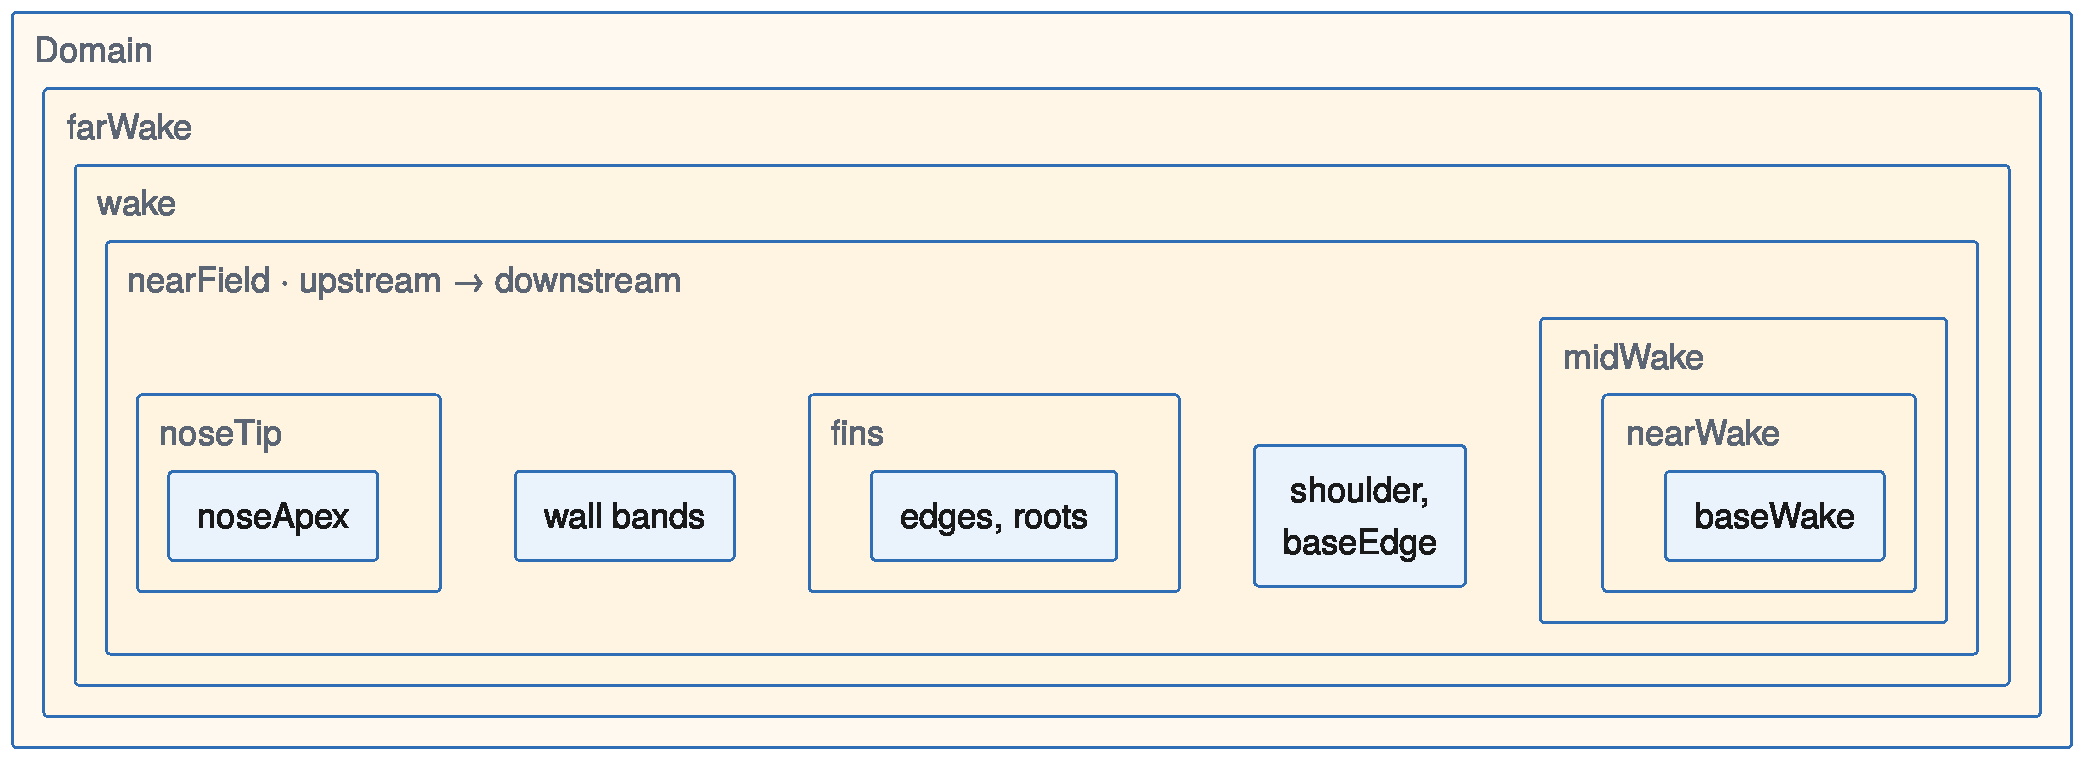
\includegraphics[width=\linewidth]{figures/pdf/refinement.pdf}
  \caption{Nesting of the refinement regions, upstream to downstream.}
  \label{fig:refinement}
\end{figure}

\begin{longtable}{@{}P{0.26\linewidth} P{0.66\linewidth}@{}}
\caption{Function of each refinement and the principle that sets its level.}\label{tab:regions}\\
\toprule
Refinement & What it resolves, and the principle \\
\midrule
\endfirsthead
\toprule
Refinement & What it resolves, and the principle \\
\midrule
\endhead
\ent{localRefinement}: \val{cone}, \val{walls}, \val{tail} & A band of thickness \ent{refinementThickness} along each wall. It contains the boundary layer and, on the nose, the region between the wall and the bow shock. The surface cell size also sets the layer thickness (\cref{sec:layers}). \\
\ent{localRefinement}: \val{fins} & The fin chord. A finer level than the body, because the fin is thin and its edges carry the strongest gradients. \\
\ent{edgeMeshRefinement}: \val{finEdges} & The leading edge (stagnation point, attached or detached shock) and the trailing edge (expansion). \\
\ent{edgeMeshRefinement}: \val{finRoots} & The fin-body junction, where the boundary layers of two walls meet. \\
\val{noseTip}, \val{noseApex} & The curvature of the nose tip: the cell must be smaller than the local radius of curvature, and the layers thinner than it. \\
\val{shoulder}, \val{baseEdge} & The expansion over the boattail and the separation at the base edge, where the base shear layer starts. They set the base pressure. \\
\val{baseWake}, \val{nearWake}, \val{midWake} & The base recirculation and the shear layer, one level coarser in each region downstream, as the wake spreads and its gradients decrease. \\
\val{nearField}, \val{wake}, \val{farWake} & Transition from the body to \ent{maxCellSize}, so that the level changes gradually. \\
\bottomrule
\end{longtable}

The regions are written as fractions of the body: each coordinate along $x$ is
multiplied by \ent{lBody}, and each coordinate across by \ent{rBody}, both from
\file{meshInfo}. The regions thus follow a rocket of another size.

The wake regions are cones on the body axis. At an angle of attack $\alpha$ the wake
moves by $\tan\alpha$ for each unit length downstream. Make sure that the wake stays
inside the wake regions over the length that sets the base pressure, for the largest
angle of the study.

\begin{caution}
\cmd{foamDictionary -set} evaluates the \texttt{\#eval} entries of \file{meshDict} and
writes numbers. \file{Allmesh} writes \ent{lBody} and \ent{rBody} with \cmd{sed}
first, for this reason. Do not set \ent{lBody} with \cmd{foamDictionary}.
\end{caution}

\section{Boundary layers}\label{sec:layers}

cfMesh extrudes the layers from the surface mesh. The thickness of the first cell
$t_1$ thus comes from the surface cell size $h$, the number of layers $n$
(\ent{nLayers}) and the growth ratio $r$ (\ent{thicknessRatio}):
\[
  t_1 \propto h\,\frac{r - 1}{r^{\,n} - 1}.
\]
\cmd{cartesianMesh} makes the layer thinner than this rule by a constant factor, so the
rule gives equal $t_1$ on meshes with equal right-hand side, but not the value of $t_1$.

\paragraph{Principle.} In a mesh study, keep $t_1$ equal on all meshes. If $t_1$
changes, \yplus{} changes, and the study mixes the change of the wall treatment with
the discretization error. As $h$ decreases from mesh to mesh, decrease $n$ or adjust
$r$ so that the rule gives the same value. \file{meshes.txt} gives $n$ and $r$ for each
mesh. Measure $t_1$ on each new mesh:
\begin{shell}
./post/firstLayer.py <mesh-dir>
\end{shell}
It gives $y$, the distance from the centre of the first cell to the wall (as
\ent{yPlus} uses it), and $t_1 = 2y$, for each wall patch, weighted by the face area.

\paragraph{Estimate of \yplus.} The mesh does not set \yplus. Estimate it before a
study from the flat-plate friction at the aft body, where \yplus{} is lowest:
\[
  Re_x = \frac{U_\infty x}{\nu_\infty},\qquad
  C_f \approx 0.0576\,Re_x^{-1/5},\qquad
  u_\tau = U_\infty\sqrt{C_f/2},\qquad
  y^+ = \frac{y\,u_\tau}{\nu}.
\]
\yplus{} grows with the speed, so one mesh gives the first cell in the viscous
sublayer at low Mach numbers and in the buffer or log layer at high Mach numbers. The
wall function of $\nu_t$ must then be valid for all \yplus{} (\cref{sec:wall-treatment}).
Measure \yplus{} on each run (\cref{sec:outputs}).

\paragraph{Layers only on wall patches.} cfMesh splits the layer only on the patches
with an entry in \ent{patchBoundaryLayers}. The global \ent{nLayers} is for the domain
faces. Keep an entry for each wall patch.

\paragraph{Fins.} The fins have fewer layers than the body
(\ent{patchBoundaryLayers/fins}). A thin fin cannot hold a thick layer stack: the
layers of the two faces meet. \ent{allowDiscontinuity} lets the number of layers change
at the fin-body junction.

\section{Domain}\label{sec:domain}

\file{Allmesh} sets the domain with \cmd{surfaceGenerateBoundingBox}, from distances to
the bounding box of the rocket. The upstream and downstream distances are fixed in
\file{Allmesh}; the lateral walls are at a fixed distance from the axis for any rocket,
so the box is symmetric about $z = 0$.

\begin{tabularx}{\linewidth}{@{}P{0.20\linewidth} L@{}}
\toprule
Boundary & Principle \\
\midrule
Upstream & In subsonic flow the disturbance of the body decays with the distance; the inlet must be far enough that the free-stream condition is correct there. In supersonic flow the inlet must be upstream of the bow shock. \\
Lateral & In subsonic flow, small blockage. In supersonic flow, the Mach cone from the nose, at the angle $\mu = \arcsin(1/M)$, exits through the lateral boundary, so that boundary needs a non-reflecting condition (\cref{sec:bc}). \\
Downstream & The outlet must be far behind the base recirculation, so that no flow enters through it. \\
\bottomrule
\end{tabularx}

\begin{caution}
\file{Allmesh} calculates the lateral distances with \cmd{awk} and sets
\cmd{LC_ALL=C}. In a locale with a decimal comma, \cmd{awk} writes numbers that
OpenFOAM reads incorrectly (\cref{sec:ts-locale}).
\end{caution}

\section{Half mesh}\label{sec:half-mesh}

If the fins have a plane of symmetry that contains the free-stream velocity, half the
domain is sufficient. By default \file{Allmesh} turns the fins so that $z = 0$ is such
a plane, meshes the whole rocket, and keeps the half $z \geq 0$:

\begin{steps}
\item The domain box is symmetric about $z = 0$, so the octree has faces on that
  plane and the cells do not cross it.
\item \cmd{topoSet} and \cmd{subsetMesh} keep the cells with the centre at $z \geq 0$.
\item \file{snapPlane.py} moves the points of the cut onto $z = 0$. The smoothing of
  \cmd{cartesianMesh} leaves them slightly off the plane.
\item \cmd{createPatch} makes the cut the patch \val{symm}, of type \val{symmetry}.
\item \file{meshInfo} gets \ent{sector half} and half the reference area, so the
  coefficients are those of the full rocket. The flow can then have an angle of
  attack in the $x$--$y$ plane, but no sideslip.
\end{steps}

\begin{caution}
Do not mesh the half domain directly, with a domain face on $z = 0$. \cmd{cartesianMesh}
treats that face as a domain boundary that touches the wall: it extrudes wall layers
into it, and the layers fan out at the corner.
\end{caution}

\section{Patches}

\cmd{createPatch} merges the six faces of the box into \val{inlet}, \val{outlet} and
\val{box}, of type \val{patch}. The \file{.fms} surface gives no type to its patches,
so \cmd{cartesianMesh} makes all of them \val{wall}; after \cmd{createPatch}, only the
rocket patches stay \val{wall}. The wall functions and the \ent{yPlus} function object
need this type. \file{Allmesh} stops if a patch in \ent{wallPatches} is not \val{wall}.

\paragraph{Feature edges.} \cmd{surfaceFeatureEdges} marks an edge as a feature edge
when the angle between the two adjacent triangles exceeds a limit. \cmd{cartesianMesh}
moves vertices onto these edges. Set the limit above the facet angle of the rounded
edges, so that only the real edges of the box and the nose are features. A low limit
marks false edges where the facets of a round are small, and the cells bend along them.

\section{meshInfo}\label{sec:meshinfo}

File: \file{mesh/meshInfo}. \file{Allmesh} copies it into the mesh directory and adds
the record of the mesh; \file{newCase.sh} copies it into the case.

\begin{longtable}{@{}P{0.28\linewidth} P{0.18\linewidth} P{0.46\linewidth}@{}}
\caption{Entries of \texttt{meshInfo}.}\label{tab:meshinfo}\\
\toprule
Entry & Written by & Function \\
\midrule
\endfirsthead
\toprule
Entry & Written by & Function \\
\midrule
\endhead
\ent{sector}, \ent{symmetryFraction} & user, \file{Allmesh} & Part of the rocket in the mesh. \file{Allrun} checks the flow angles against it. \\
\ent{Aref}, \ent{lRef} & user, \file{Allmesh} & Reference area (scaled with the sector) and length of the coefficients. \\
\ent{rBody}, \ent{lBody} & user & Scale the refinement regions. \\
\ent{fins}, \ent{finRootR}, \ent{finTipR}, \ent{finX0}, \ent{finX1} & user & Fin data for \file{Allrefine}. \\
\ent{wallPatches} & user & Patches in the force integration. \\
\ent{nCells}, \ent{maxCellSize}, \ent{finLevel}, \ent{nLayers}, \ent{thicknessRatio}, \ent{meshDir} & \file{Allmesh} & Record of the mesh. \\
\bottomrule
\end{longtable}

\section{Make a mesh}\label{sec:allmesh}

\begin{shell}
mesh/Allmesh <mesh-dir> [stl-file] [--maxCellSize <m>] [--nLayers <n>]
             [--thicknessRatio <r>] [--full]
\end{shell}

The options write into the copy of \file{meshDict}; the options that you do not give
keep the values of \file{mesh/system/meshDict}. Without \ent{--full} the mesh is a half
mesh. \file{Allmesh} does not write into a directory that exists.

\begin{figure}[htbp]
  \centering
  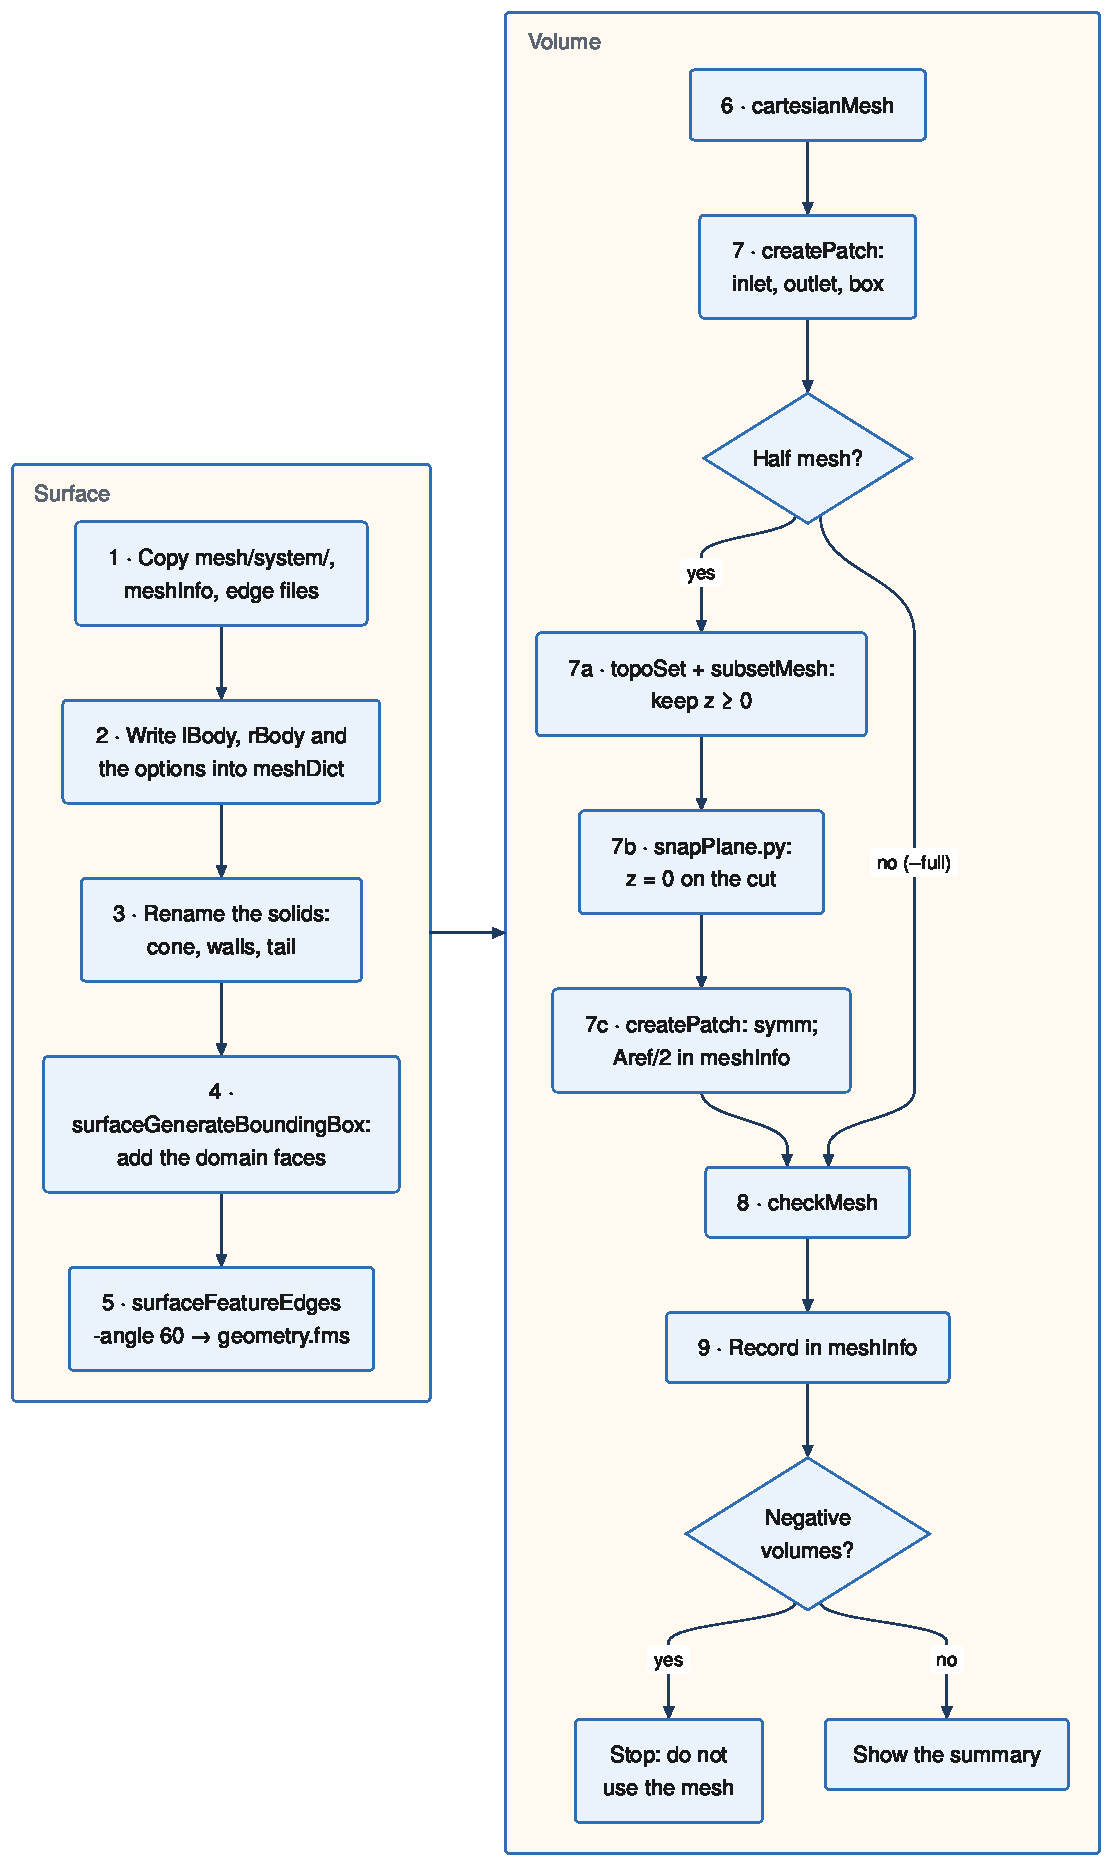
\includegraphics[width=0.85\linewidth,height=0.8\textheight,keepaspectratio]{figures/pdf/allmesh.pdf}
  \caption{Steps of \texttt{Allmesh}: surface operations, then volume operations.}
  \label{fig:allmesh}
\end{figure}

\file{Allmesh} reads the log of each application and stops on \val{FOAM FATAL}, because
\cmd{runApplication} returns 0 also when an application fails.

\section{Examine a mesh}\label{sec:examine-mesh}

\begin{steps}
\item Read the summary of \file{Allmesh}. A mesh with negative cell volumes is not
  usable: change the geometry or \file{meshDict}, and make a new mesh.
\item Examine the patch types in \file{constant/polyMesh/boundary}.
\item Measure $t_1$ with \file{post/firstLayer.py}, and compare it with the other
  meshes of the study.
\item Look at the cells on the fin edges, the base edge and the boattail shoulder in
  ParaView.
\end{steps}

\begin{note}
\cmd{checkMesh -allGeometry} also reports small determinants in layer cells, face tets
and concave cells. These checks are of a different category from negative volumes and
do not stop the use of the mesh. Record them with the mesh.
\end{note}
